\chapter{Active Galactic Nuclei}
\label{chap:Active Galactic Nuclei}
\section{Overview of AGNs}
As technology improved throughout the 20th century, astronomers were able to observe the universe in different ways, discover new objects and phenomena that were unknown. Discoveries such as the cosmic microwave background and pulsars revolutionized our understanding of the universe and the laws of physics that apply to it.

The third major discovery, often mentioned alongside the cosmic microwave background and pulsars, is that of Active Galactic Nuclei, specifically quasars (``Quasi-stellar radio sources''), first introduced by \citet{10.1063/1.3051610}.

Active Galactic Nuclei are some of the most powerful and luminous objects in the universe and can outshine entire galaxies within a fantastically small volume. The energy output of these objects is so high that it is difficult to understand how they can produce it. The consensus is that this energy is produced by the accretion of matter onto a supermassive black hole, which typically has a mass ranging from $10^6$ to $10^{10}$ $\text{M}_\odot$.

AGNs have diverse regions emitting different types of radiation. It is usually in the literature that we find the following components \citep{RadiativeProcesses}:

\begin{itemize}
    \item \textbf{The Supermassive Black Hole:} A black hole whose origin is still a source of speculation, but one which is believed to have emerged in the early universe. Its mass is $10^6 - 10^{10}$ solar masses, and is the source of the energy output in AGNs.
    \item \textbf{The Accretion Disk:} A ring-shaped mass of matter surrounding the black hole, slowly being accreted into it. Matter in the disk is heated to temperatures ranging from tens of thousands to millions of degrees, depending on a multitude of factors, such as the black hole's mass and the region of the Disk. This heated matter produces radiation across the entire electromagnetic spectrum.
    \item \textbf{The Corona:} A region of hot, ionized gas located outside the accretion disk and believed to be the source of the X-ray emission in AGNs.
    \item \textbf{The Obscuring Torus:} A structure, likely toroidal or clumpy, composed of gas and dust that encircles the accretion disk and absorbs a portion of the radiation emitted, subsequently re-emitting it in the infrared region.
    \item \textbf{The Broad Line Region:} A region consisting of ionized gas formed by a number of small, fast-moving clouds in close proximity to the accretion disk. Doppler shifts broaden the observed lines, giving the region its characteristic name.
    \item \textbf{The Narrow Line Region:} Another region of ionized gas at a larger distance from the accretion disk, where less dense clouds are moving, less rapidly. The lower velocities of this region lead to narrower spectral lines.
    \item \textbf{The Jet:} About 10\% of observed AGNs launch collimated jets of highly energetic particles, likely ejected from the poles of the black hole at relativistic velocities. Their appearance depends on the viewing angle. AGNs whose jets are pointing at us are called blazars. AGNs whose jets are pointing elsewhere are typically classified as radio galaxies.
\end{itemize}

Figure \ref{fig:AGN_structure} illustrates the schematic structure of an AGN.

\begin{figure}[H]
    \centering
    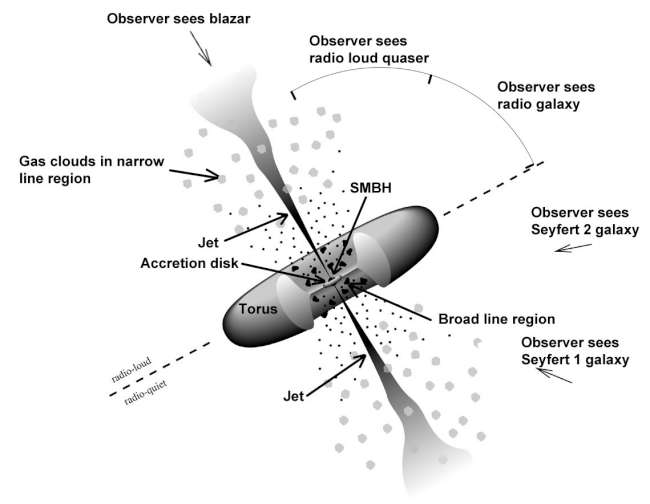
\includegraphics[width=0.65\textwidth]{Figures/AGN Structure.jpg}
    \caption{The general structure of an Active Galactic Nucleus. The different regions mentioned before are labeled. Figure taken from \url{https://fermi.gsfc.nasa.gov/science/eteu/agn/}}
    \label{fig:AGN_structure}
\end{figure}


\section{Radiation Mechanisms in AGNs}

As stated, the main topic of this project is the production of gamma rays in the AGN of NGC 1068 and how they interact with the surrounding gas and radiation. We should first try to understand the underlying mechanisms that produce this type of radiation as well as all the types of radiation at play in such regions.

It is also essential to make a distinction between thermal and non-thermal emission processes. Thermal emission has its origin in hot matter in the AGN. It follows a blackbody-like distribution, and is produced by particles which are in thermal equilibrium. Non-thermal emission, on the other hand, is produced by particles that are not in thermal equilibrium and are accelerated to high energies, thus producing radiation through different processes.


In general, AGNs emit the following types of radiation \citep{RadiativeProcesses}:

\begin{itemize}
    \item \textbf{Radio Emission:}
    \subitem \textbf{Synchrotron Radiation:} It is generated by relativistic electrons moving in magnetic fields, which is common in AGN jets and lobes. In these sources, the spectrum typically covers photon energies from approximately $10^{-9}$ eV up to about $10^{-5}$ eV. In powerful radio-loud AGNs, this component can be extremely luminous, sometimes exceeding $10^{24}$ W Hz$^{-1}$.
    \subitem \textbf{Free-Free Emission:} Generated by the interaction of free electrons with ions in the gas, which is common in HII regions (regions of ionized hydrogen).
    \subitem \textbf{Maser Emission:} In some AGNs, molecules such as water in dense regions produce amplified microwave signals. This emission is typically observed around $10^{-6}$ eV and, while striking, generally represents only a minor fraction of the overall radio luminosity.
    
    \item \textbf{Infrared Emission:}
    \subitem \textbf{Thermal Dust Emission:} Dust in the circumnuclear torus absorbs high-energy photons and re-emits them as energy in the infrared. The resulting spectrum spans energies from 0.001 to 1 eV. In obscured AGNs, this infrared component can dominate the bolometric output.
    
    \item \textbf{Optical/UV Emission:}
    \subitem \textbf{Thermal Emission:} The inner parts of the accretion disk surrounding the supermassive black hole are heated to temperatures high enough to emit thermal radiation that peaks in the optical/UV band. This emission typically spans photon energies from about 1 eV to 10 eV, and in many unobscured AGNs it is the dominant contributor to the total luminosity.
    \subitem \textbf{Broad and Narrow Line Emission:} In addition to the continuum, ionized gas in the broad-line and narrow-line regions produces characteristic spectral lines in the optical/UV. As an example, we have the H$_{\alpha}$ line at 6563 \AA\ (about 1.89 eV).
    
    \item \textbf{X-ray Emission:}
    \subitem \textbf{Non-thermal Emission:} Relativistic electrons, primarily in the corona (upscattering disk photons) and potentially in jets, produce X-rays via inverse Compton scattering, typically in the 0.1 keV to 100 keV range.
    
    \subitem \textbf{Bremsstrahlung:} In certain AGNs, collisions in the hot gas produce thermal X-ray emission, which generally occurs over a similar energy interval (roughly 0.1 - 100 keV). Although significant, this process usually contributes less to the total X-ray luminosity than the non-thermal component.
    
    \item \textbf{Gamma-ray Emission:}
    \subitem \textbf{Inverse Compton Scattering:} In the AGN's jets, high-energy electrons collide with low-energy background photons, boosting them to gamma-ray energies. This mechanism typically yields gamma rays in the range of 100 keV up to more than 10 GeV, and in some blazars, it forms a major part of the high-energy emission.
    \subitem \textbf{Proton-Proton Interactions:} High-energy protons interacting with ambient protons can produce pions that decay into gamma rays (and neutrinos), often extending the spectrum into the TeV range (above $10^{12}$ eV). 
    \subitem \textbf{Proton-Photon Interactions:} Similarly, interactions between high-energy protons and low-energy photons lead to pion production and subsequent gamma-ray emission, further extending the high-energy tail into the TeV regime.
\end{itemize}

All in all, we get a complex distribution of energies in the AGN, with different processes producing different kinds of radiation. The overall resulting distribution of energies can be shown in what is known as a spectral energy distribution (SED) plot, which shows the luminosity of the AGN as a function of frequency. Figure \ref{fig:AGN_SED} shows a schematic representation of the expected SED of a general AGN (excluding the radio and microwave bands, which are not shown).

\begin{figure}[H]
    \centering
    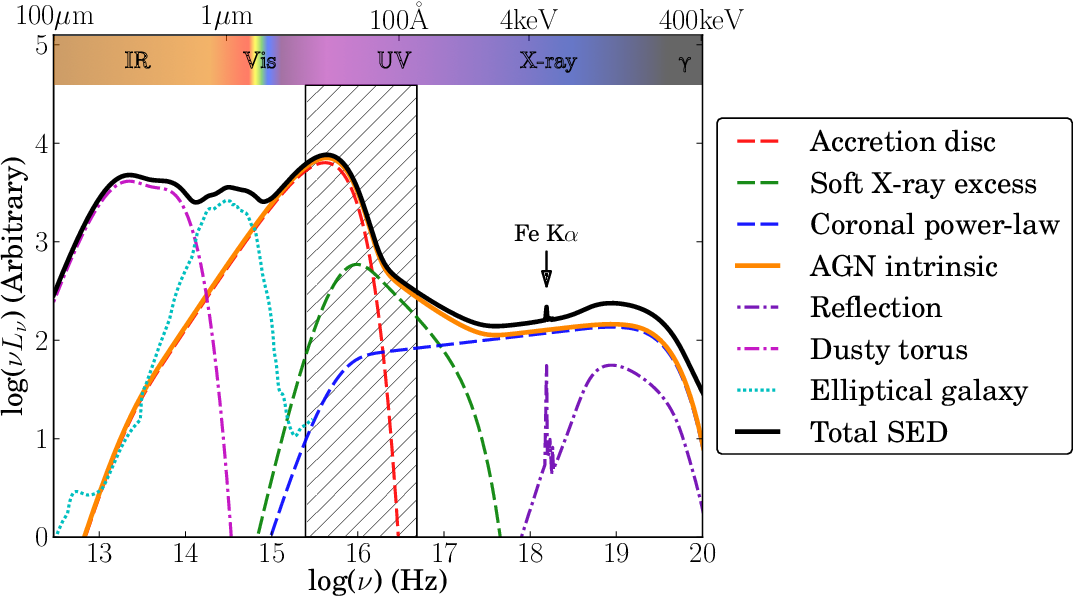
\includegraphics[width=0.9\textwidth]{Figures/AGN SED.png}
    \caption{A simplified schematic diagram of an AGN SED, showing the approximate shape and extent of the various components discussed in the text. Dashed lines denote AGN intrinsic emission, dash-dot lines show emission reprocessed by the surrounding material, and the dotted line shows starlight from an elliptical host galaxy. The hatched region highlights a spectral range often subject to significant absorption by the Intergalactic medium (IGM). The example shows contributions from an elliptical host galaxy; galaxies with active star formation would exhibit stronger UV/IR components from stars and dust. Figure adapted from \citet{QuasarSEDCollinson_2016}.}
    \label{fig:AGN_SED}
\end{figure}

Proton-proton interactions and proton-photon interactions in the AGN of NGC 1068 are of special interest, since these processes also produce neutrinos, whose energy spectrum is related to the gamma-ray spectrum in a clear and predictable manner.


\section{Gamma-ray and Neutrino Production in AGNs}

We will focus on proton-proton and proton-photon interactions, which are sources of this type of radiation in AGNs.

Inside AGNs, close to the supermassive black hole, we find a region of hot, ionized gas, which is mainly composed of protons and electrons. These particles are accelerated to very high energies by mechanisms such as diffusive shock acceleration or magnetic reconnection \citep{padovani2024highenergyneutrinosvicinitysupermassive}. The accelerated protons can then collide with other protons or photons in the gas, producing pions through the simplified processes specified below:


\begin{figure}[H]
    \centering
    \feynmandiagram [large, horizontal=a to b] {
        i1 [particle=\(p\)] -- [fermion] a,
        i2 [particle=\(\gamma\)]-- [photon] a,
        a -- c [blob, label=\(\Delta(1232)\)] -- b,
        b -- [fermion] f1 [particle=\(\pi^+\text{, }\pi^0\)],
        b -- [fermion] f2 [particle=\(n\text{, }p\)],
    };
    \caption{Simplified diagram for resonant proton-photon ($p\gamma$) interaction via the $\Delta(1232)$ resonance. Near resonance, the primary channels are $p\gamma \rightarrow \Delta^+ \rightarrow n\pi^+$ (approx. $\nicefrac{2}{3}$ probability) and $p\gamma \rightarrow \Delta^+ \rightarrow p\pi^0$ (approx. $\nicefrac{1}{3}$ probability).}
  \end{figure}

\begin{figure}[H]
  \centering
  \feynmandiagram [ large, horizontal=a to b] {
      i1 [particle=\(p\)] -- [fermion] a,
      i2 [particle=\(p\)]-- [fermion] a,
      a -- c [blob, fill=blue!30] -- b,
      b -- [fermion] f1 [particle=\(p\)],
      b -- [fermion] f2 [particle=\(n\text{, }p\)],
      b -- [fermion] f3 [particle = \(\pi^+\text{, }\pi^0\)],
  };
  \caption{Simplified scheme for proton-proton interactions. The underlying interaction is represented by the blue circle.}

\end{figure}

The pions produced then decay into gamma rays and neutrinos through the following processes:
\begin{figure}[H]
    \centering
    \begin{subfigure}{0.45\textwidth}
        \centering
        \feynmandiagram [medium, vertical=a to t1] {
            a [particle=\(\pi^{0}\)] -- [scalar] t1 [blob] -- [anti fermion, edge label'=\(k^-\)] t2 -- [anti fermion, edge label'=\(k^+\)] t3 -- [anti fermion, edge label'=\(k^+\)] t1,
            t2 -- [photon, blue] p1 [blue, particle=\(\gamma\)],
            t3 -- [photon, blue] p2 [blue, particle=\(\gamma\)],
            p1 -- [opacity=0] p2,
        };
        \caption{Neutral pion decay.}
    \end{subfigure}
    \begin{subfigure}{0.45\textwidth}
        \centering
        % Using the layered layout
        \feynmandiagram [layered layout, horizontal=k to b] {
        p [particle=\(\pi^{+}\)] -- [anti fermion] a [particle=\(\mu^{+}\)],
        p -- [red, fermion] d [red, particle=\(\nu_{\mu}\)],
        a  -- [anti fermion] b -- [red, anti fermion] f1 [red, particle=\(\overline \nu_{\mu}\)],
            b -- [boson, edge label'=\(W^{+}\)] c,
            c -- [red, fermion] f2 [red, particle=\(\nu_{e}\)],
            c -- [anti fermion] f3 [particle=\(e^{+}\)],
            };
        \caption{Charged pion decay.}
    \end{subfigure}
  \end{figure}

As highlighted in blue and red, the pions decay into gamma rays and neutrinos, respectively.

Crucially, since both gamma rays (from $\pi^0$ decay) and neutrinos (from $\pi^\pm$ decay) originate from the same hadronic interactions, the neutrino flux detected from NGC 1068 implies an associated gamma-ray flux produced in the same source. The relationship between the fluxes is complex, but basic estimates suggest comparable energy outputs  \citep{M_cke_1999}. This is of great importance, since we can use the flux measured from the neutrinos as our initial estimate for the flux of gamma rays inside the AGN.

\section{Case Study: The AGN of NGC 1068}

NGC 1068 is a Seyfert type II galaxy located in the constellation Cetus, approximately 33 million light-years away from Earth\footnote{More on this value later \citep{padovani2024highenergyneutrinosvicinitysupermassive}.}. It is one of the closest AGNs to our galaxy, and has been the subject of numerous studies due to its unique properties. \citep{2MASS}

The publication of neutrino data from the IceCube collaboration \citep{IceCube2022} has sparked numerous studies on the gamma-ray and neutrino emission from NGC 1068. Turning our attention to the SED of NGC 1068, we can see in Figure \ref{fig:NGC1068_SED} that the gamma-ray emission, which should be comparable to the neutrino emission, is considerably lower.\\

In the figure, several features are highlighted: 
\begin{enumerate}
    \item The $\nu^{-0.7}$ radio spectrum.
    \item A template for emission of the host galaxy.
    \item A template for the accretion disk plus X-ray corona emission.
    \item The $\gamma$-ray and neutrino bands.
\end{enumerate}

Thus, the objective of this work will be to construct a model which can ``shift'' the energies from the neutrino spectrum to a distribution which is in agreement with the data points presented by Fermi-LAT and MAGIC.

\begin{figure}[H]
    \centering
    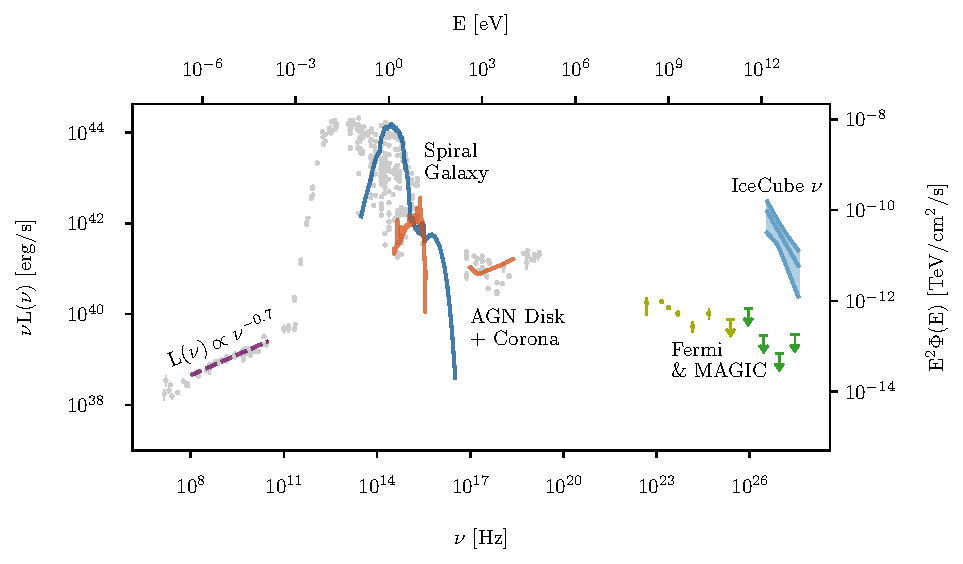
\includegraphics[width=\textwidth]{Figures/NGC1068_SED.pdf}
    \caption{The integrated multi-messenger SED of NGC 1068, assembled using the
    SED builder at the SSDC (\url{https://tools.ssdc.asi.it/SED/}), showing the power emitted at different frequencies/energies; various components are highlighted. Note that the SED tool provides multiple values at the same frequency, which reflect the different resolutions used by the facilities which have studied the source on various spatial scales. For clarity we have kept mainly the highest flux values, which are associated with the largest scales, since the SED is dominated by the host galaxy given its relatively small distance. Figure taken from \cite{padovani2024highenergyneutrinosvicinitysupermassive}.}
    \label{fig:NGC1068_SED}
\end{figure}

\section{Neutrino Detection Techniques - IceCube}
\label{sec:Neutrino_Detection}

The process of detecting neutrinos is an essential part of this project, as data obtained from the IceCube Neutrino Observatory will be used as our initial flux estimate of gamma-rays inside the AGN's corona.

The detection of neutrinos originating from distant astrophysical sources like NGC 1068 presents considerable experimental challenges due to their incredibly weak interaction with matter. This property, while making them near-perfect messengers of cosmic events, requires the construction of large-scale detectors in order to be able to detect them consistently.

The IceCube Neutrino Observatory, located at the geographic South Pole, represents the current state-of-the-art in high-energy neutrino detection \citep{IceCubeOverview2017}. It utilizes a cubic kilometer of the deep, Antarctic glacial ice as both the target material and the detection medium. Embedded in the ice is an array of over 5,000 so-called Digital Optical Modules (DOMs): highly sensitive photodetectors encased in spherical glass pressure vessels. These DOMs are arranged on 86 vertical strings, deployed at depths between 1,450 and 2,450 meters. A schematic layout of the detector can be seen in Figure \ref{fig:IceCube_layout}.

\begin{figure}[H]
    \centering
    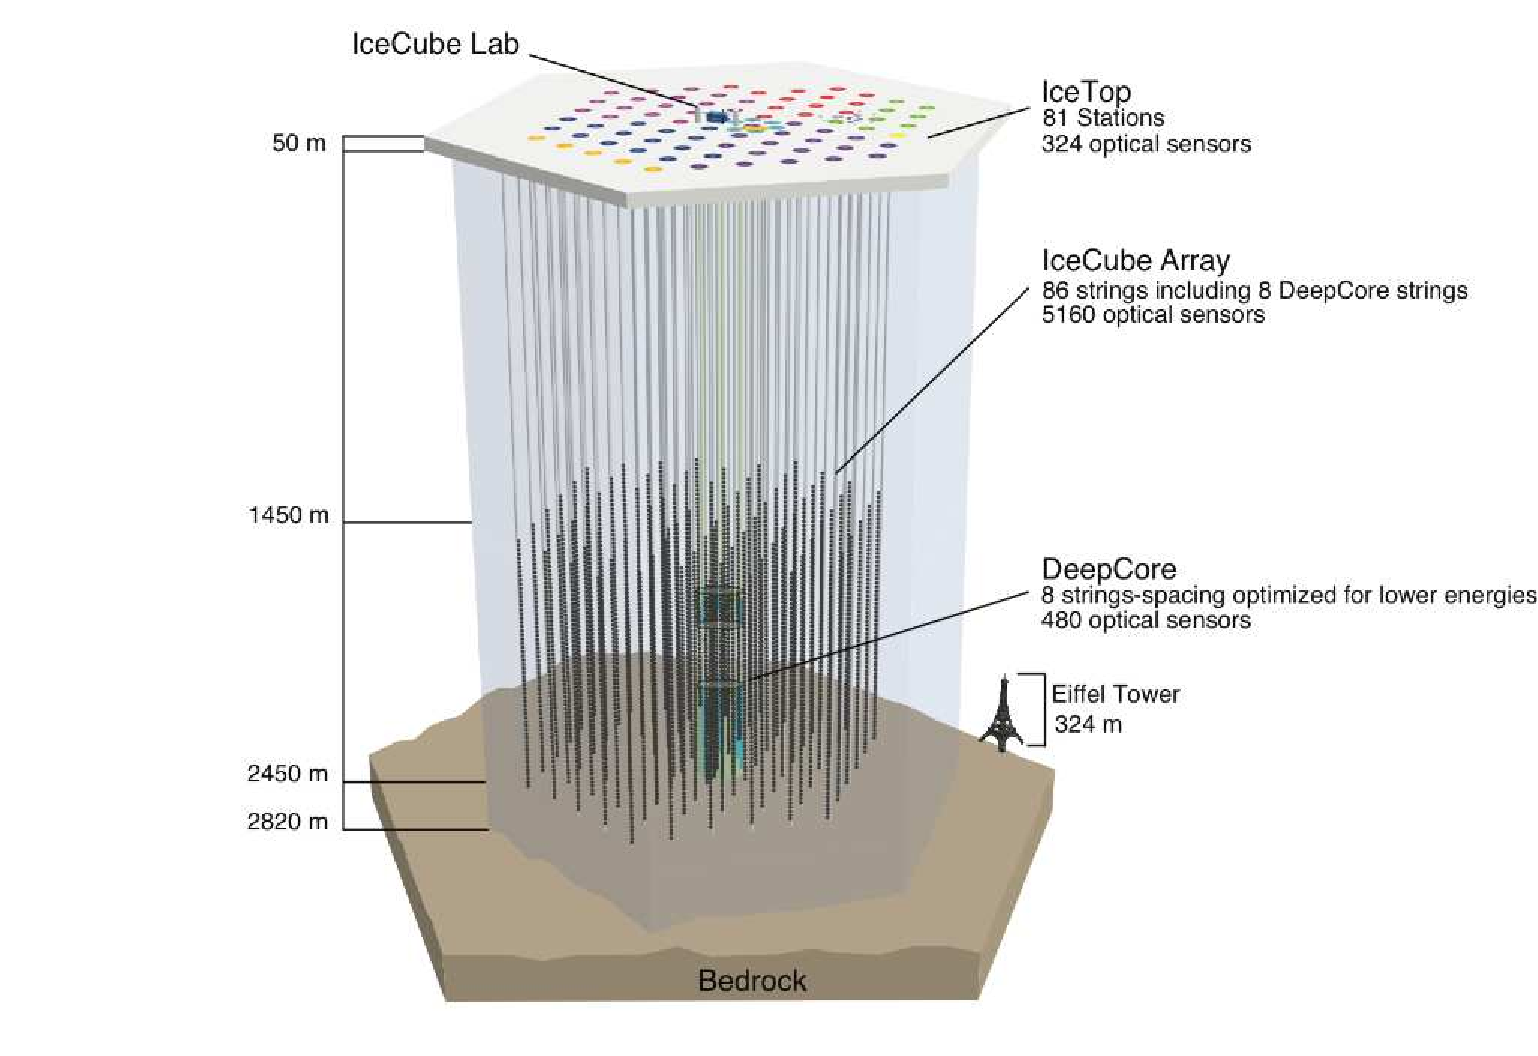
\includegraphics[width=0.9\textwidth]{Figures/IceCube_Layout.pdf}
    \caption{Schematic diagram illustrating the layout of the IceCube Neutrino Observatory beneath the Antarctic ice. The array consists of numerous vertical strings equipped with Digital Optical Modules (DOMs). Figure taken from \citet{IceCubeOverview2017}.}
    \label{fig:IceCube_layout}
\end{figure}


The detection principle which IceCube exploits relies on observing the Cherenkov radiation produced by secondary charged particles generated when a neutrino interacts within or near the instrumented ice volume. A high-energy neutrino ($ \nu_l $, where $ l = e, \mu, \tau $) can interact with a nucleon (N) in an ice molecule via charged-current (CC) or neutral-current (NC) weak interactions:
\begin{itemize}
    \item Charged Current (CC): $ \nu_l + N \rightarrow l + X $
    \item Neutral Current (NC): $ \nu_l + N \rightarrow \nu_l + X $
\end{itemize}
where $l$ is the corresponding charged lepton (electron, muon, or tau) and $X$ represents the resulting hadronic system.

If the charged secondary particles produced (the lepton $l$ in CC interactions, or particles within the hadronic cascade $X$) travel through the ice faster than the speed of light in that medium ($c/n$, where $n \approx 1.31$ is the refractive index of ice), they emit Cherenkov radiation. This radiation manifests as a cone of faint blue light propagating through the ice, depicted conceptually in Figure \ref{fig:Cherenkov_cone}. The DOMs detect the timing and intensity of this light.

\begin{figure}[H]
    \centering
    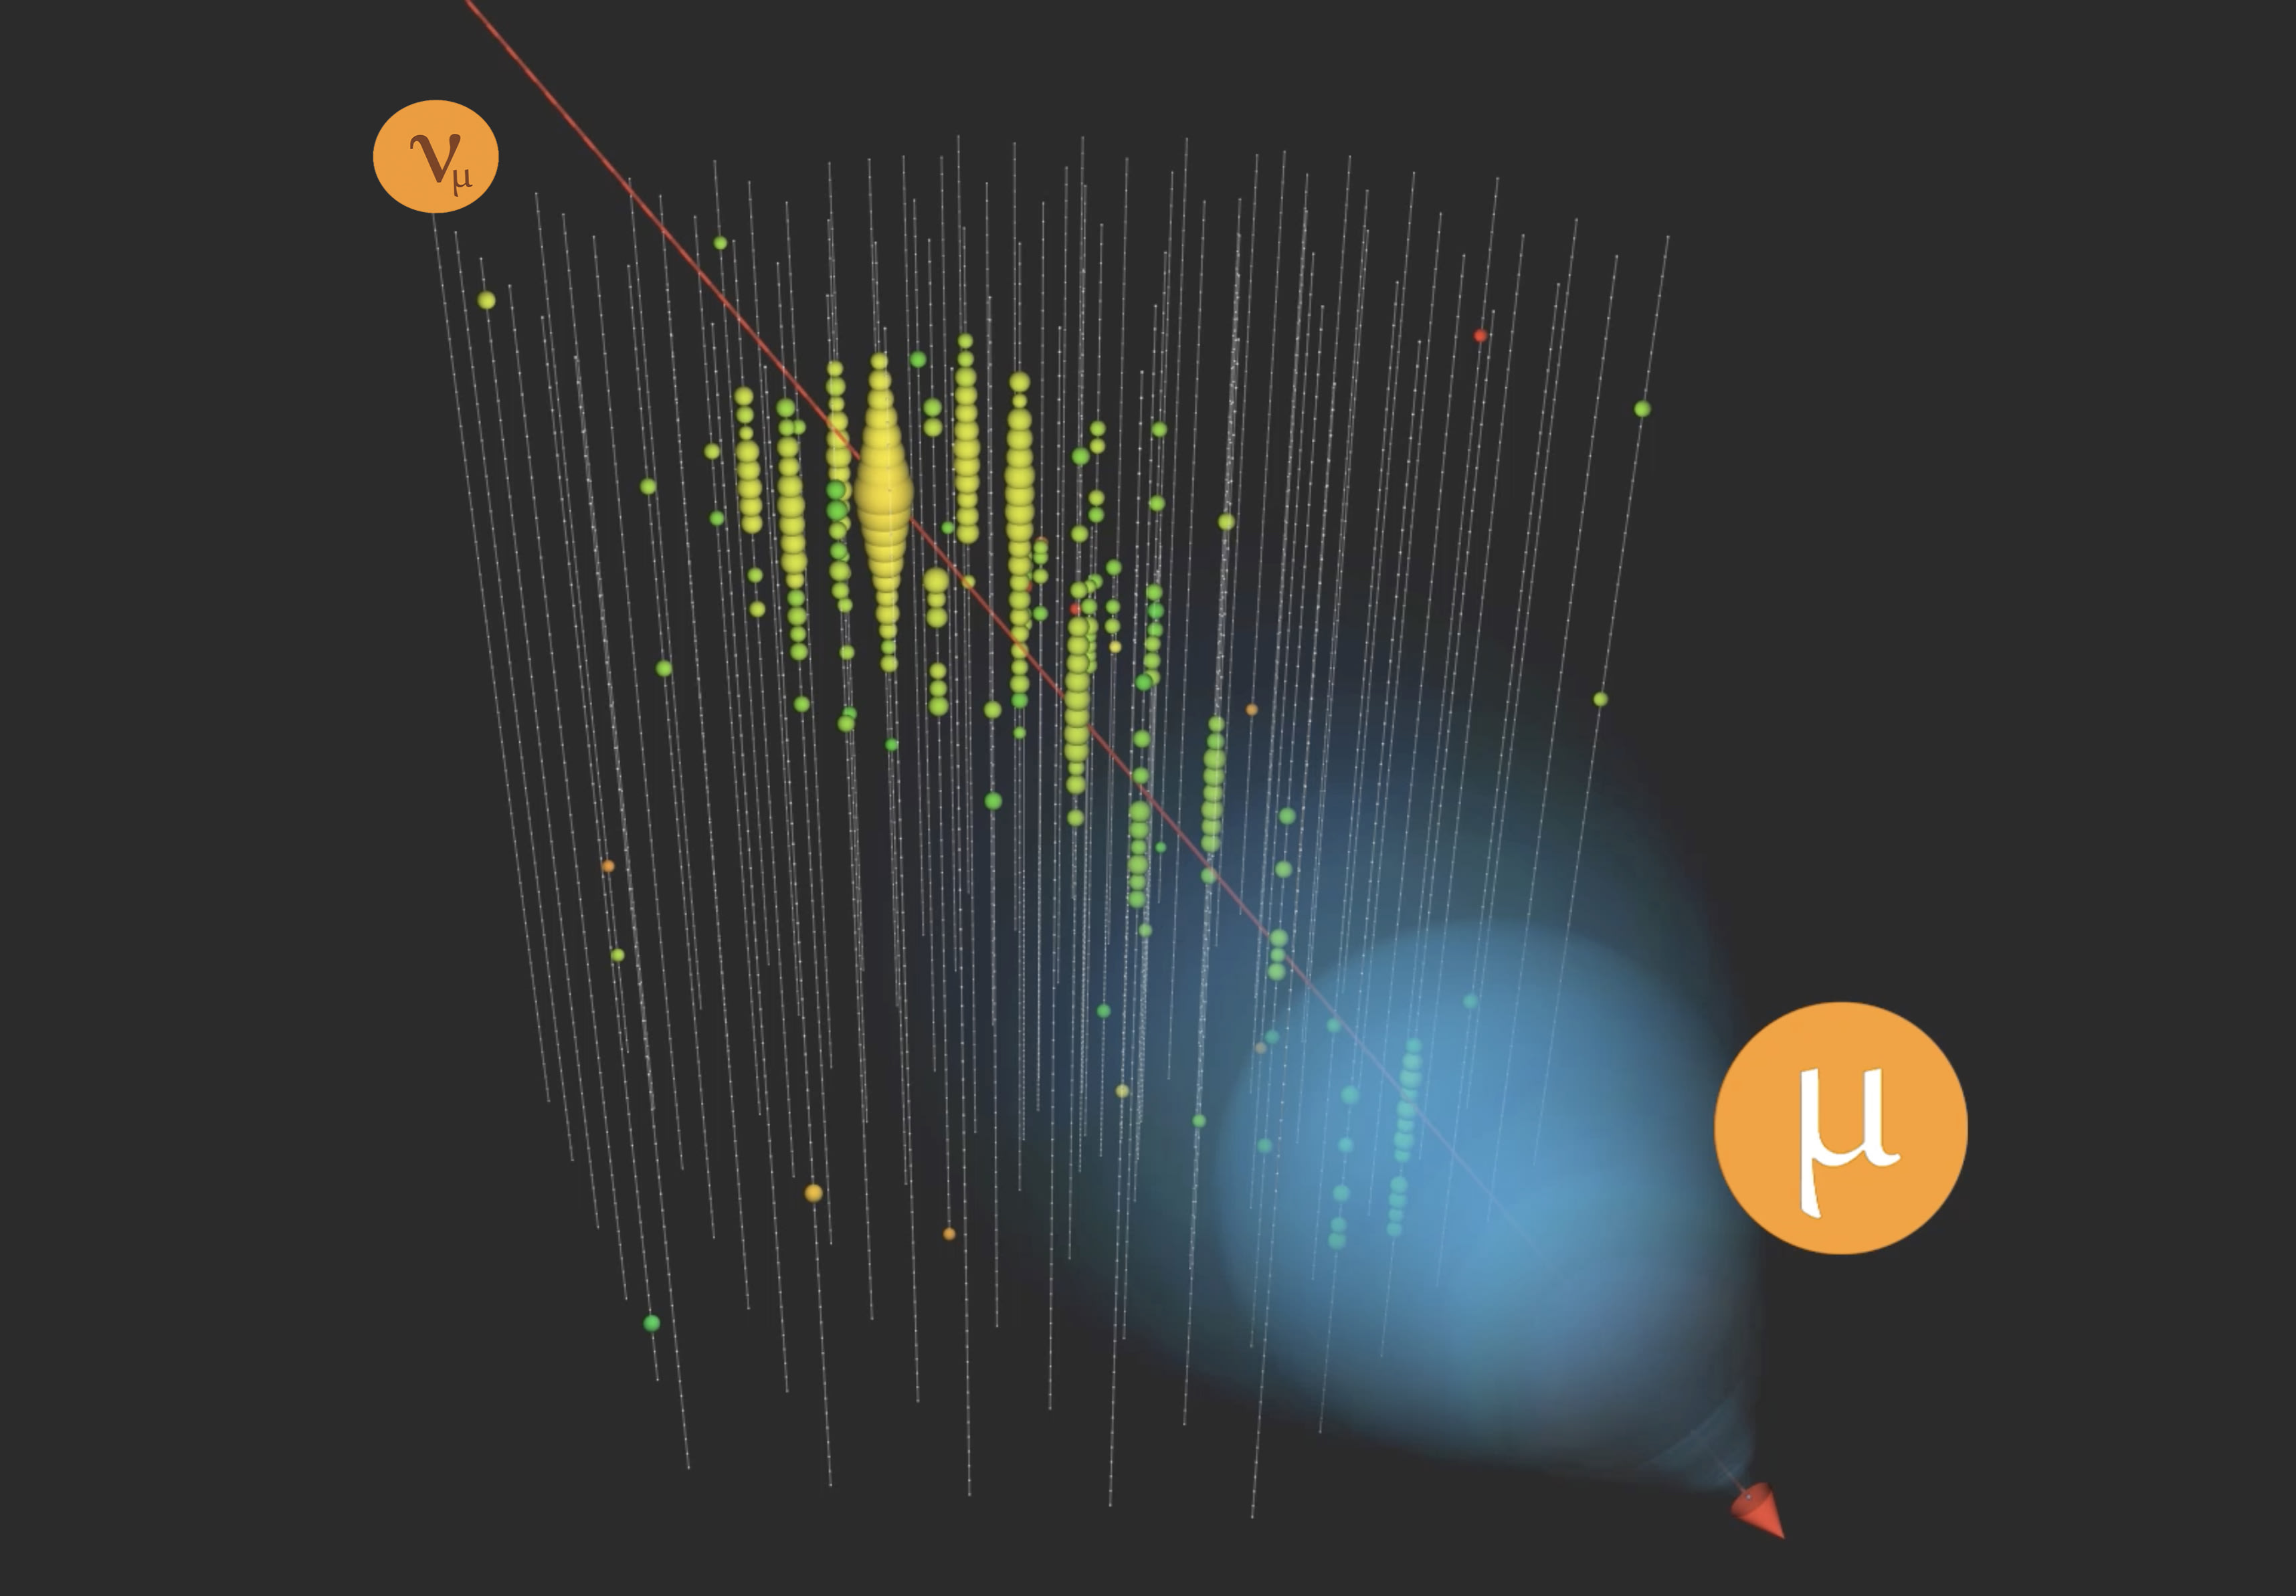
\includegraphics[width=0.8\textwidth]{Figures/Cherenkov.jpg}
    \caption{Conceptual illustration of Cherenkov radiation emitted by a muonic neutrino traveling faster than the speed of light in the ice medium. The light propagates in a cone, which is detected by the DOMs. Figure taken from \url{https://icecube.wisc.edu/gallery/measuring-the-neutrino-cross-section-with-earth-absorption/}}
    \label{fig:Cherenkov_cone}
\end{figure}


The shape of the detected light pattern allows for the classification of neutrino events and the reconstruction of their properties. Two primary event topologies are observed:
\begin{itemize}
    \item \textbf{Tracks:} Primarily produced by muons generated in $ \nu_{\mu} $ CC interactions ($ \nu_{\mu} + N \rightarrow \mu + X $). High-energy muons can travel several kilometers through the ice, producing long, linear tracks of Cherenkov light. The extended nature of these tracks allows for a relatively precise reconstruction of the muon's (and thus the incident neutrino's) direction, typically achieving sub-degree angular resolution for high-energy events. An example of a track event is shown in Figure \ref{fig:Track_event}.
    \item \textbf{Cascades (or Showers):} Result from $ \nu_e $ CC interactions ($ \nu_e + N \rightarrow e^- + X $), $ \nu_{\tau} $ CC interactions ($ \nu_{\tau} + N \rightarrow \tau + X $, where the tau lepton decays rapidly), and NC interactions of all neutrino flavors. In these events, the energy is deposited more locally, creating electromagnetic and/or hadronic showers. The resulting Cherenkov light pattern is roughly spherical or elliptical and more contained. Cascades generally provide better energy resolution compared to tracks, as more of the initial neutrino energy is deposited within the detector volume, but offer poorer angular resolution (typically around $10^\circ - 15^\circ$). Figure \ref{fig:Cascade_event} shows an example of a cascade.
\end{itemize}


\begin{figure}[H]
    \centering
    \begin{subfigure}{0.48\textwidth}
        \centering
        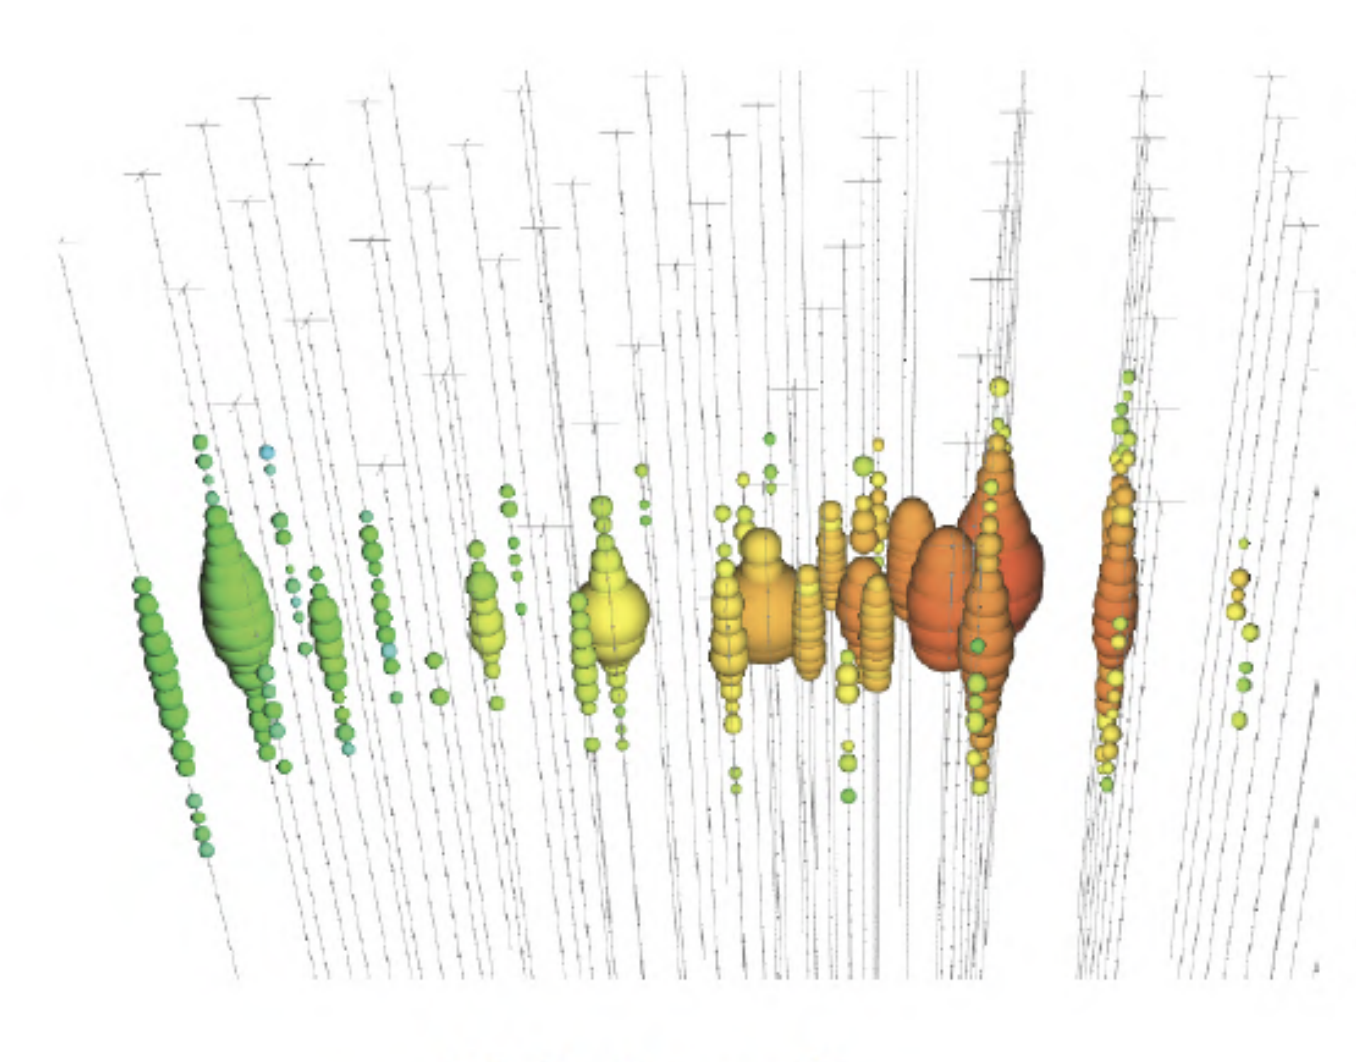
\includegraphics[width=\textwidth]{Figures/Track.png}
        \caption{Example event display of a muon track signature in IceCube. The colored spheres represent DOMs, with color indicating arrival time and size indicating light intensity. The linear pattern allows for directional reconstruction.}
        \label{fig:Track_event}
    \end{subfigure}
    \hfill
    \begin{subfigure}{0.48\textwidth}
        \centering
        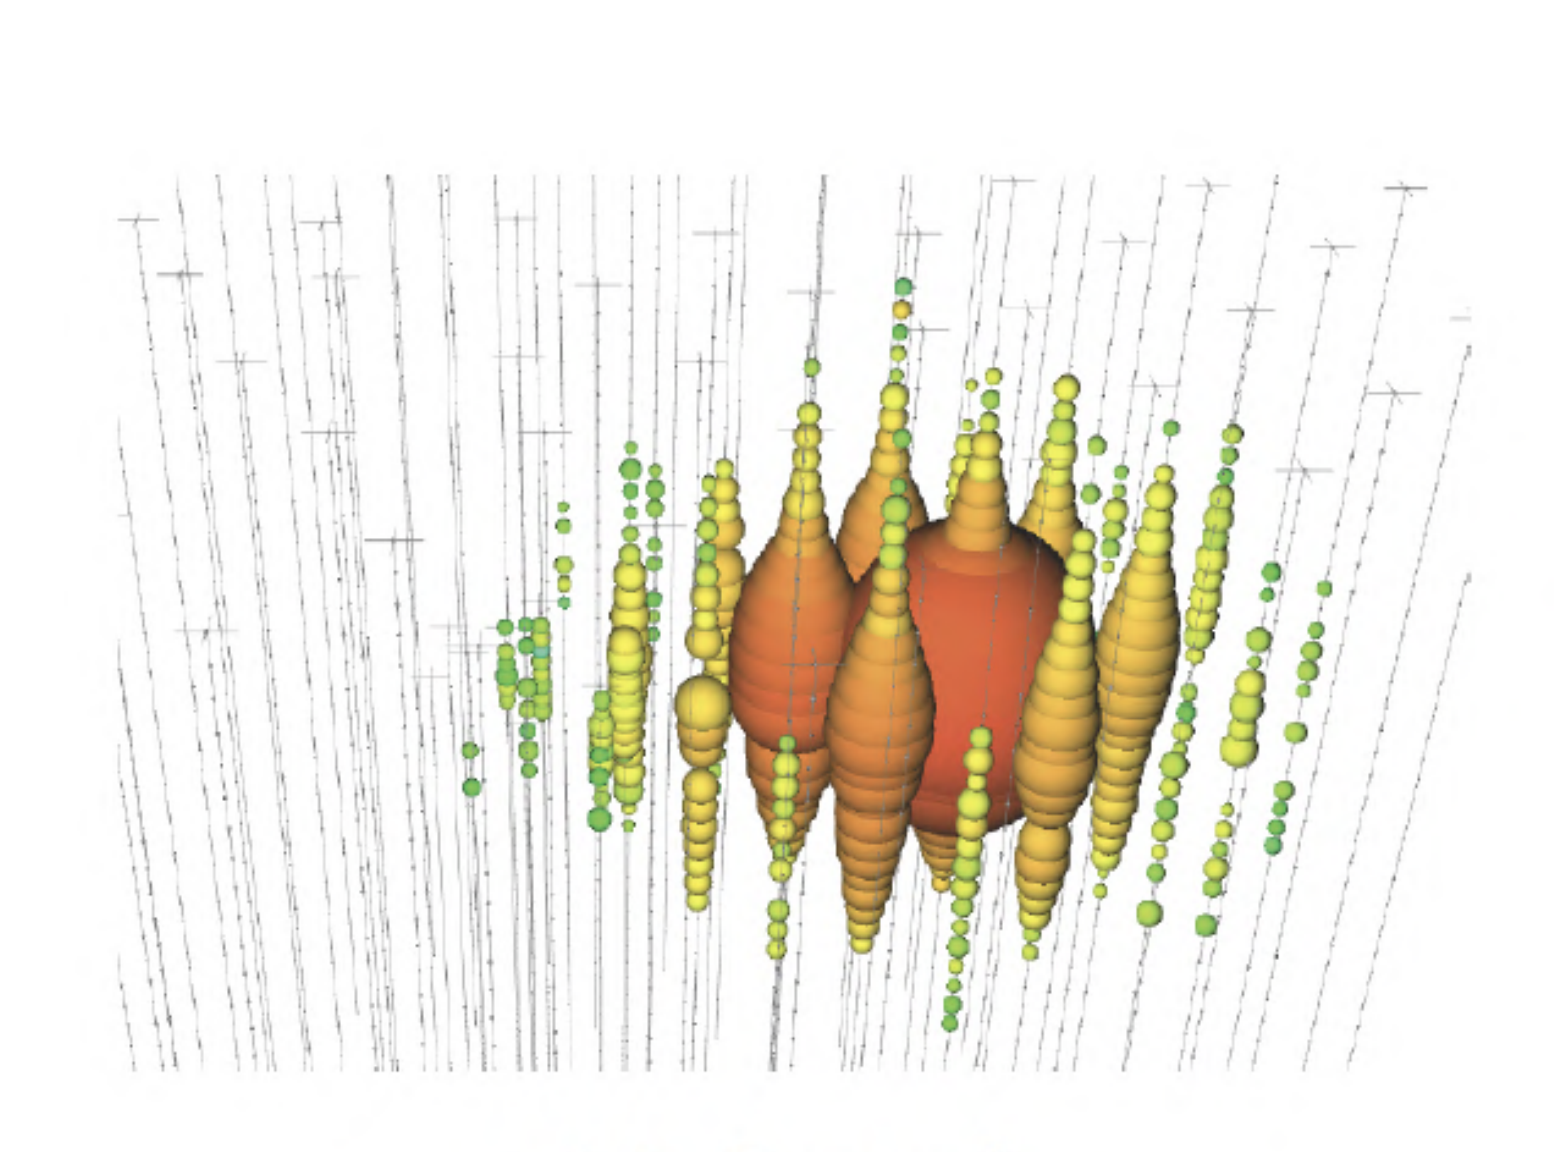
\includegraphics[width=\textwidth]{Figures/Cascade.png}
        \caption{Example event display of a cascade signature in IceCube. The light is deposited more locally compared to a track, providing good energy information but poorer directional information.}
        \label{fig:Cascade_event}
    \end{subfigure}
    \caption{Typical event topologies observed in the IceCube detector. Figures taken from \citet{Kowalski_2017}}
    \label{fig:Event_topologies}
\end{figure}


By analyzing the spatio-temporal pattern of the light recorded by the DOMs, reconstruction algorithms determine the event's topology, estimate the neutrino's energy, and reconstruct its arrival direction. This directional data is essential for identifying potential astrophysical sources, such as the AGN of NGC 1068, by searching for statistically significant excesses of events clustered in specific regions of the sky above the large background of atmospheric neutrinos and muons. The detection of high-energy neutrinos coincident with known astrophysical objects offers strong proof for hadronic acceleration processes occurring within them.


%The background section should give sufficient background information to give the reader an overview of the state-of-the-art research field in which you work.

%The background chapter can be a bit similar to the introduction. For journal articles, it is not that common with a background section, as it is not kept separate from the introduction. However, for a master thesis, it is common to have more background and therefore to separate out some of the background material into a separate chapter. For a specialization project, the background chapter could be the most important chapter, as the specialization project is centered around learning a new subject field.

%Do not overestimate the background knowledge of the reader. As a rule of thumb, you could assume (s)he knows as much as you did when you started on your master thesis/project. So you need to give the reader enough background to be able to read the rest of your thesis.

%All relevant literature should be included, so do a thorough literature search. When you do, try not to miss out on the classics and defining papers in your field of work. For a specialization project, your background section can include references to display the breadth of the field you are working on. In contrast, for a master thesis, you should be able to argue for all included references. Do not add references just to get a long reference list. After you have spent a lot of time reading something, it could be tempting to add those references to just show off that you have read them, even though it turned out after reading them that it is not fully related to your work. Do not, all included references in your master thesis should be relevant to your work.

%The background material should also motivate your work. It should make your research question interesting by showing what others have done, and showing what is missing, highlighting the void that you try to fill with your work.


%\section{Citations}

%The background needs relevant literature to place your project work into context. The Google-scholar search (\url{scholar.google.com}) is a good starting point for searching for relevant papers.  This subsection will show how to include these references in your latex-document.

%There is a long range of different styles and packages in Latex for citations. During your writing process, it is often beneficial to have an \texttt{authoryear} style, where you see the author(s) and the year of publication. This will help you remember what the reference is. In the \texttt{main.tex} file you will find a command defining the bibliography style.

%This is where you want to go to change the style of your referencing. In this setup, we use the \texttt{natbib} style. This allows for using \verb=\citep= and \verb=\citet= references, which are useful if you use \texttt{authoryear} style:
%\begin{itemize}
 %   \item Whenever the reference is part of the sentence, you should use the textual citation \verb=\citet=. The \verb=\citet= reference types will give a reference that looks like this: \citet{berg2014permeability}.
 %   \item Whenever the reference is not a part of the sentence, but just general for the sentence or paragraph, you should use the parenthetical citation \verb=\citep=. The \verb=\citep= reference types will give a reference that looks like this: \citep{berg2014permeability}.
 %   \item If you do not specify, but use \verb=\cite=, it will look like this: \cite{berg2014permeability}.
%\end{itemize}

%All the references you use will automatically show up in your reference list. If you want to shift to numerical citations, you should use the \texttt{cite} command, as there are no differences between textual and parenthetical citations when you use the numerical style.

